% GENERATED by reporting/make_tsae_report.py -- do not edit by hand.
% Source: metrics/outputs/{toy-temporal,gemma-2-2b*}/ -- frozen run results, not prose.
% Every caption is TODO on purpose: a caption is a claim about what to take away,
% and this project requires those to be written by a person.
% Regenerate:  python3 -m reporting.make_tsae_report
% Requires:    \input{thresholds_macros.tex} in the preamble (defines \MinJoint etc.),
%              and packages booktabs, graphicx, amsmath.


% ------------------------------------------------------------------------
% Toy model
% ------------------------------------------------------------------------

% [toy-decorr]
\begin{figure}[tbp]
  \centering
  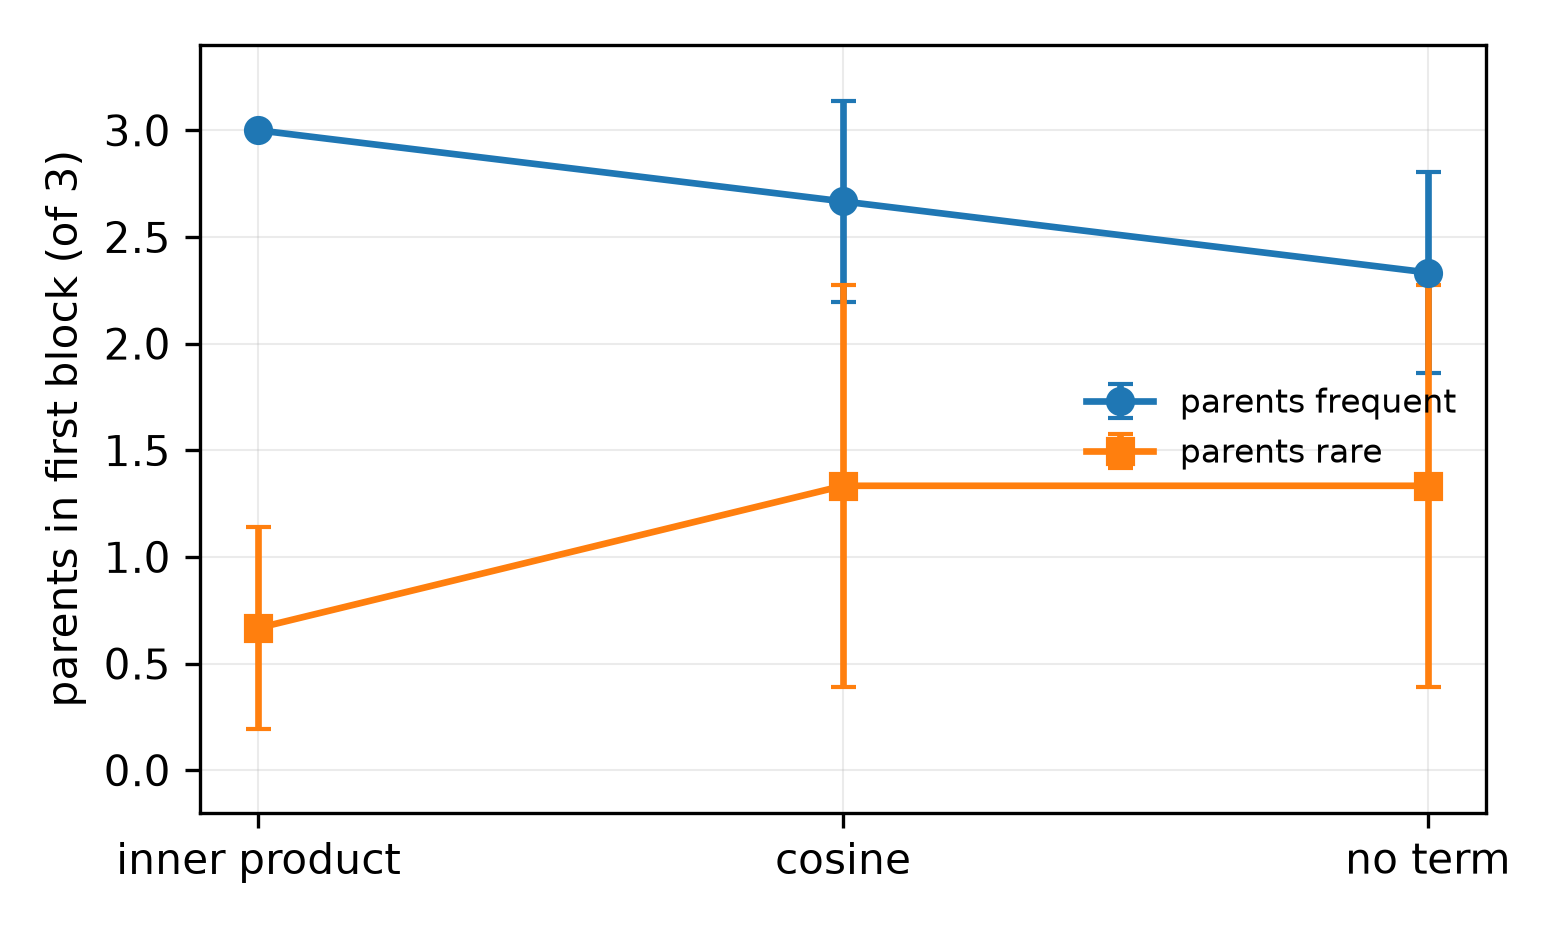
\includegraphics[width=0.62\linewidth]{figuers/tsae_decorrelated_parents}
  \caption{TODO(caption, human-written). How many parents land in the first block, on the two worlds. The bars show the average of three runs. The lines through them show how much the three runs differed from each other.}
  \label{fig:tsae-decorrelated-parents}
\end{figure}

% ------------------------------------------------------------------------
% gemma-2-2b layer 12
% ------------------------------------------------------------------------

% [thresholds]
\begin{figure}[tbp]
  \centering
  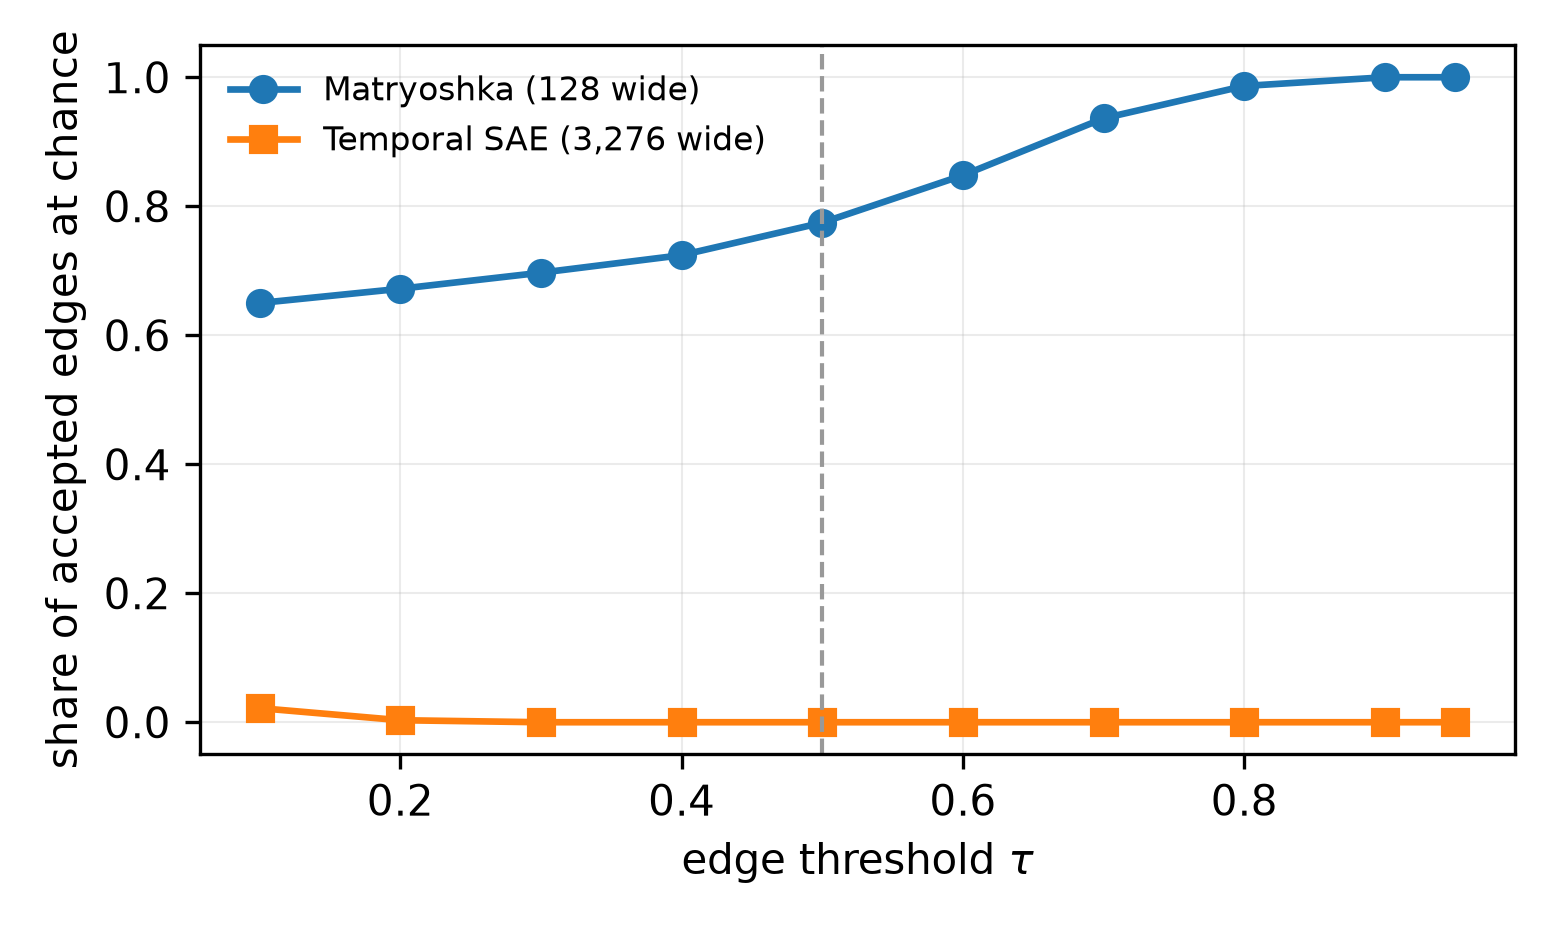
\includegraphics[width=0.62\linewidth]{figuers/tsae_threshold_reversal}
  \caption{TODO(caption, human-written). The same cut-off, drawn. Going right means a stricter cut-off. Going up means more of the surviving links could be explained by the two features simply being common. The dashed line is the setting we use everywhere else in this paper.}
  \label{fig:tsae-threshold-reversal}
\end{figure}
